\chapter{ ГЛАВА 1. ОПИСАНИЕ МОДЕЛИРУЕМЫХ ФИЗИЧЕСКИХ ЯВЛЕНИЙ}
\label{ch:chapter1}
\section{Распределение Максвелла-Больцмана}
Если система находится в состоянии равновесия, то средние значения любых ее параметров не будут зависеть от времени. Поэтому функция распределения должна зависеть только от интегралов движения системы. Основным интегралом движения является полная механическая энергия системы $E$ или функция Гамильтона $H$. Соответсвенно простейший общий вид функции распределения будет $w(x)=w(H)$. Конкретный же вид этой функции $w(H)$ нужно определить. Функция Гамильтона зависит от $6N$ переменных системы $x$ и от внешних параметров $a$, т. е. $H(x,a)$. \cite{physstat69}

Для идеального газа функцию  Гамильтона $H(x,a)$ можно просто заменить энергией $E(x)$, тогда по формуле канонического распределения Гиббса для изотермической системы
$$w(x)=e^{\frac{\psi - H(x, a)}{\theta}} \eqno (1.1.1)$$
вероятность нахождения системы с энергией $E$ в элементе фазового пространства $(dx)^{6N}$ будет

$$dW(x)=e^{\frac{\psi - E}{\theta}}=const \: e^{-\frac{E}{kT}}(dx)^{6N}. \eqno (1.1.2)$$

Для системы невзаимодействующих частиц энергию $E$ можно представить как сумму энергий отдельных частиц $E=\sum_{i=1}^{N} E_i$. Тогда вероятность (1.1.1) можно разбить на $N$ сомножителей

$$dW(x)=const \: e^{-\frac{E_i}{kT}}dx_1dy_1dz_1dp_{x_1}dp_{y_1}dp_{z_1}...$$

$$...e^{-\frac{E_N}{kT}}dx_Ndy_Ndz_Ndp_{x_N}dp_{y_N}dp_{z_N}. \eqno (1.1.3)$$

\noindent Интегрируя по $6(N-1)$ переменной всех частиц, кроме $i$-й, получим выражение вероятностей для $i$-й частицы:

$$dW(x_i,y_i,z_ip_{xi}p_{yi}p_{zi})=const \: e^{-\frac{E_i}{kT}}dx_idy_idz_idp_{x_i}dp_{y_i}dp_{z_i} \eqno (1.1.4)$$

\noindent Здесь $E_i$ рассматривается как функция $6$ переменных $p_{x_i}$, $p_{y_i}$, $p_{z_i}$, $x_i$, $y_i$, $z_i$. Распределение (1.2.4) можно рассматривать в $6$-мерном фазовом пространстве одной молекулы, которое называют $\mu$-пространством ($\mu - $ от слова молекула). \cite{physstat69}

\noindent Энергия отдельной частицы $E_i$ может быть представлена суммой кинетической и потенциальной энергий, зависящих от импульса и координат частицы, соответственно:

$$E=E_{\text{кин}}+E_{\text{пот}}=\frac{p_{x}^2+p_{y}^2+p_{z}^2}{2m}+ U(x,y,z)\eqno(1.1.5)$$

\noindent Подставляя это выражение в (1.1.4), получим

$$dW(p_x,p_y,p_z, x,y,z)=const \: e^{-\frac{\frac{p_{x}^2+p_{y}^2+p_{z}^2}{2m}+ U(x,y,z)}{kT}}dp_xdp_ydp_zdxdydz. \eqno (1.1.6)$$

\noindent Это и есть распределение Максвелла$-$Больцмана.

Тот факт, что кинетическая и потенциальная энергии зависят от разных переменных, дает возможность рассмотреть одно распределение (1.1.6) как два независимых распределения в трехмерном пространстве импульсов и в трехмерном пространстве координат:

$$dW(p_x,p_y,p_z)=Ae^{-\frac{p_{x}^2+p_{y}^2+p_{z}^2}{2mkT}}dp_xdp_ydp_z, \eqno (1.1.7)$$

$$dW(x,y,z)=Be^{-\frac{U(x,y,z)}{kT}}dxdydz. \eqno (1.1.8)$$
Здесь $A$ и $B$  постоянные, определяемые из условия нормировки распределений. Функция распределения по координатам частицы (1.1.8) в потенциальном поле представляет так называемое распределение Больцмана (1877 г.). \cite{physstat69}

$$dW(z)=Be^{-\frac{U(z)}{kT}}dz. \eqno (1.1.9)$$

\noindent Для идеального газа в однородном поле силы тяжести из (1.1.9) выводится известная барометрическая формула. Действительно, в этом случае $U(z)=mgz$ и функция распределения частиц по высоте $z=h$ принимает вид

$$f(z)=\frac{dW(z)}{dz}=Be^{-\frac{mgz}{kT}}. \eqno (1.1.10)$$

\noindent Вследствие пропорциональности числа частиц $n(z)$ функции распределения (1.1.10) получим следующее распределение числа частиц в единице объема по высоте $z$:

$$n(z)=const \: e^{-\frac{mgz}{kT}}.$$

\noindent Поскольку при $z=0$ в единице объема будет $n_0$ частиц, то для распределения частиц по высоте получим

$$n(z)= n_0 e^{-\frac{mgz}{kT}}. \eqno (1.1.11)$$

\noindent Если учесть, что в газе давление пропорционально плотности, то из (1.1.11) получается барометрическая формула

$$\rho(z)= \rho_0 e^{-\frac{mgz}{kT}}. \eqno (1.1.12)$$

Экспериментальные исследования показали, что на больших высотах в атмосфере наблюдаются отклонения числа частиц от распределения, описываемого формулой (1.1.11), связанные с неоднородным составом атмосферы, с различием температур на разных высотах и с тем, что атмосфера не находится в состоянии равновесия.
В атмосферах планет происходит явление рассеяния атмосферы в космическое пространство. Оно объясняется тем, что всякая частица, имеющая скорость больше второй космической для данной планеты, может покинуть атмосферу планеты. В газе, как следует из максвелловского распределения, всегда имеется некоторая доля молекул с очень большими скоростями, уход которых и определяет постепенное рассеяние верхних слоев атмосферы. Рассеяние атмосферы планет происходит тем быстрее, чем меньше масса планеты и выше ее температура.

Для Земли этот эффект оказывается ничтожно малым, а планета Меркурий и Луна уже потеряли таким способом свои атмосферы.

\section{Распределение Максвелла}
Рассмотрим поступательное движение частиц максвелл-больцмановского идеального газа, пренебрегая квантованием энергии. Из формул распределения Максвелла-Больцмана

$$dN=e^{(\mu - \epsilon)/kT} \frac{d\text{Г}}{h^f}, \eqno (1.2.1)$$

$$N=\int e^{(\mu - \epsilon)/kT} \,\frac{d\text{Г}}{h^f} \eqno (1.2.2)$$

\noindent получаем выражение для вероятности нахождения изображающей точки в элементе объема $d\text{Г}$-пространства

$$ dW=\frac{dN}{N}=\frac{e^{- \epsilon/kT}d\text{Г}}{\int e^{- \epsilon/kT}\,d\text{Г}}, \eqno (1.2.3)$$

\noindent где выражение, стоящее в знаменателе, есть статистический интеграл $Z$. \cite{termkin72} Мы будем рассматривать газ, состоящий из молекул с произвольным числом $n$ атомов в молекуле. Поскольку, однако, нас интересует сейчас только поступательное движение, мы выделим из всех обобщенных координат и импульсов молекулы три координаты центра масс $(x, y, z)$ и соответствующие им проекции полного импульса молекулы $(\xi,\eta, \zeta)$, и представим энергию молекулы в виде

$$\epsilon = \frac{\rho^2}{2m}+U(x,y,z)+\epsilon' \eqno (1.2.4)$$

\noindent где $\rho^2=\xi^2 + \eta^2 + \zeta^2$ $-$ квадрат импульса молекулы как целого, $U(x, y, z)$ $-$ потенциальная энергия молекулы во внешнем поле (предполагается, что она не зависит от ориентации молекулы) и $ \epsilon '$ $-$ энергия остальных степеней свободы, не зависящая от $(x, y, z,\xi,\eta, \zeta)$. Интегрируя выражение (1.2.3) по всем степеням свободы кроме поступательных, мы найдем вероятность того, что центр масс молекулы лежит в объеме $dV$, а импульс ее заключен в интервале $(\rho, \rho +d \rho)$. Эта вероятность распадается на два сомножителя: один зависит только от импульса, а другой $-$ только от координат $$ dW= \frac{e^{- \rho^2/2mkT}dV_\rho}{\int e^{- \rho^2/2mkT}\, dV_\rho} \frac{e^{- U(x,y,z)/kT}dV}{\int e^{- U(x,y,z)/kT}\, dV}.\eqno (1.2.5)$$

Это значит, что распределение молекул по импульсам и распределение их по координатам не зависят друг от друга. Интегрируя выражение (1.2.5) по координатам, получим

$$ dW(\rho)= \frac{e^{- \rho^2/2mkT}dV_\rho}{\int e^{- \rho^2/2mkT}\, dV_\rho}.\eqno (1.2.6)$$

\noindent Записав элемент объема пространства импульсов в виде $dV_p = 4\pi\rho^2d\rho$ и вычисляя интеграл, стоящий в знаменателе

$$4\pi \int_{0}^{\infty} e^{-\frac{\rho^2}{2mkT}}\rho^2\, d\rho = 4\pi J_2 =(2\pi mkT)^{3/2},$$

\noindent получим распределение молекул газа по импульсам

$$ dW(\rho)= \frac{4\pi}{(2\pi mkT)^{3/2}} e^{-\frac{\rho^2}{2mkT}}\rho^2 d\rho.\eqno (1.2.7)$$

\noindent Переходя от импульса к скорости, имеем

$$ dW(v)= 4\pi \left(\frac{m}{2\pi kT}\right)^{3/2} e^{-\frac{mv^2}{2kT}}v^2 dv.\eqno (1.2.8)$$

\noindent Формулы (1.2.7), (1.2.8) называются формулами распределения Максвелла и позволяют решать ряд конкретных задач. \cite{termkin72}

Найдем наиболее вероятную скорость молекул газа. Для этой скорости выражение (1.2.8) должно иметь максимум:

$$\frac{d}{dv}\left(v^2e^{-\frac{mv^2}{2kT}}\right)=ve^{-\frac{mv^2}{2kT}}\left( 2 - \frac{mv^2}{kT}\right)=0,$$

\noindent откуда

$$v_\text{в}=\sqrt{\frac{2kT}{m}}.\eqno (1.2.9)$$

\noindent Легко также найти среднюю и среднюю квадратичную скорость молекул

$$v=\int v\,dW(v)=4\pi \left(\frac{m}{2\pi kT}\right)^{3/2}\int_{0}^{\infty}v^3e^{-\frac{mv^2}{2kT}}\, dv= \sqrt{\frac{8kT}{\pi m}},\eqno (1.2.10)$$

$$\overline{v^2}=\int v^2\,dW(v)=4\pi \left(\frac{m}{2\pi kT}\right)^{3/2}\int_{0}^{\infty}v^4e^{-\frac{mv^2}{2kT}}\, dv= \frac{3kT}{ m}.\eqno (1.2.11)$$

\noindent Отсюда средняя энергия поступательного движения молекул равна

$$\overline{E_{\text{к}}}=\frac{m\overline{v^2}}{2}=\frac{3}{2}kT.$$

\noindent График распределения Максвелла имеет вид, изображенный на рис. 1.2.1. С повышением температуры максимум кривой смещается

 \begin{figure}[ht]
	\centering
\hspace*{\fill}%
\begin{subfigure}[b]{0.49\textwidth}
        \centering
		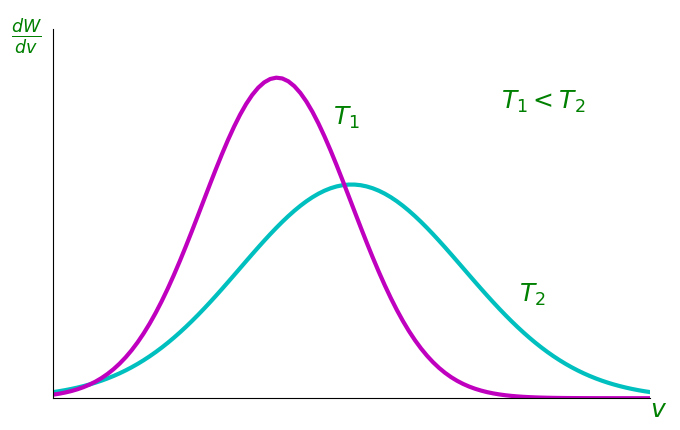
\includegraphics[height=5cm,keepaspectratio]{images/maxwell2.png}
        \caption{\textbf{Рис. 1.2.1.}}
	\end{subfigure}
	\begin{subfigure}[b]{0.49\textwidth}
        \centering
		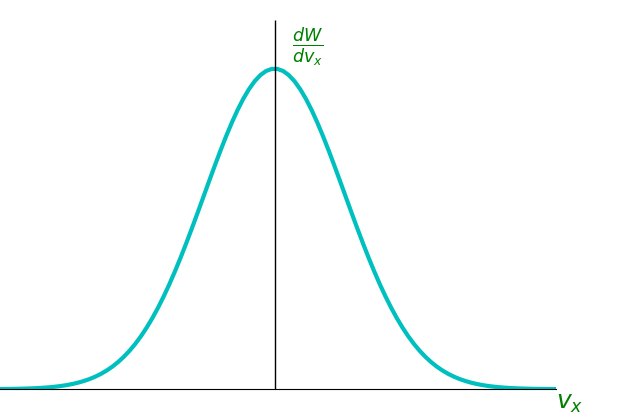
\includegraphics[height=5cm,keepaspectratio]{images/maxwell1.png}
		\caption{\textbf{Рис. 1.2.2.}}
	\end{subfigure}
 \hfill
 \hspace*{\fill}%
 \end{figure}
 \noindent в сторону высоких температур и сам график становится более пологим с более существенным «хвостом», тянущимся в область больших скоростей.

Если рассекать импульсное пространство не на шаровые слои, а на параллелепипеды $dv_x$, $dv_y$, $dv_z$, то распределение (1.2.6) можно записать в виде произведения трех множителей вида

$$dW(v_i)=\left( \frac{m}{2 \pi kT}\right)^{1/2}e^{-\frac{mv_i^2}{2kT}}dv_i\quad (i=x,y,z). \eqno (1.2.12)$$

\noindent Это свидетельствует о том, что распределения по величине разных проекций скорости независимы. График распределения Максвелла по проекциям скорости имеет вид, изображенный на рис. 1.2.2.

Нетрудно понять из физических соображений и проверить путем прямого вычисления, что среднее значение проекций $v_x$, $v_y$, $v_z$ равно нулю. Сделаем в заключение следующее замечание. Хотя мы вывели распределение Максвелла для идеального газа, оно на самом деле имеет значительно более широкую область применимости. Оно справедливо для всех систем взаимодействующих частиц, если температура настолько высока, что можно пренебрегать квантованием энергии. Это следует из того, что распределение Максвелла может быть получено из канонического распределения Гиббса, если представить энергию системы в виде $E = mv_i^2/2 + E'$, где $E'$ $-$ энергия системы (включая и энергию взаимодействия молекул) за вычетом кинетической энергии центра инерции $i$-й молекулы, и проинтегрировать функцию распределения по координатам всех молекул и по всем обобщенным скоростям, кроме скорости центра инерции $i$-й молекулы. \cite{termkin72}

\section{Броуновское движение}

Молекулярное движение приводит к диффузии, к проникновению молекул одного газа в другой.

Пусть вдоль оси $Oz$ имется градиент концетрации некоторого примесного газа в основном газе. Тогда через едничную площадку в единицу времени снизу перемещается больше молекул диффундирующего газа, а сверху (где концетрация ниже) $-$ меньше. Таким образом, возникает направленный поток газа снизу вверх. Поток газа, вызванный диффузией, удовлетворяет закону Фика
$$ I = D\frac{dc}{dz}, \eqno (1.3.1)$$

\noindent где $D$ $-$ коэффициент диффузии. \cite{physstat69}

Для вычисления этого коэффициента рассмотрим диффузионный поток газа. Снизу вверх в слой $z$ через единичную площадку за время $dt$  проходит $\frac{\overline{v}n_1dtS}{6}$ молекул диффундирующего газа, а сверху из слоя $z+l$ вниз $- \frac{\overline{v}n_2dtS}{6}$ молекул.

Из самого слоя $z$ в слои $z+l$ и $z-l$ уходит $\frac{\overline{v}n_0dtS}{3}$ молекул. Разность этих велечин дает число молекул, перемещающихся за время $dt$ через площадку $S$ в направлении от слоя $z-l$ к слою $z+l$;
$$dn = \frac{\overline{v}Sdt}{6}(n_2+n_1-2n_0).$$

\noindent Здесь $n_1$, $n_0$ и $n_2 -$ среднее число молекул в слоях $z+l$, $z$ и $z-l$, отстоящих друг от друга на расстоянии $l$ и отличающихся по числу молекул на $\Delta n = \frac{dc}{dz}l$.

\noindent Поток частиц от слоя с большей концетрацией к слою с меньшей концетрацией равен
$$l=\frac{\Delta n}{S \Delta t}= \frac{\overline{v}S\Delta t}{6S \Delta t} \cdot 2 \cdot \frac{dc}{dz}l= \frac{\overline{v}l}{3} \frac{dc}{dz}. \eqno (1.3.2)$$

\noindent А следовательно коэффициент диффузии определится соотношением
$$D=\frac{l}{\frac{dc}{dz}}= \frac{\overline{v}l}{3}. \eqno (1.3.3)$$

\noindent Здесь $\overline{v}$ $-$ средняя скорость молекул, считается независящей от концетрации и $l$ $-$ средняя длина свободного пробега. Коэффициент диффузии, таким образом, оказывается $\overline{v}$ и от давления или плотности газа через $l$. \cite{physstat69}

Эта формула для коэффициента диффузии с учетом выражения длины свободного пробега часто используется для оценки эффективного диаметра (размеров) молекул $d_0$.

Броуновское движение $-$ непрерывное, беспорядочное движение малых частиц, взвешенных в жидкости или газе, происходящее под действием ударов молекул окружающей среды. Броуновское движение представляет собой одно из наиболее ярких и доступных наблюдению проявлений молекулярно-кинетической природы хаотического теплового движения атомов и молекул.
Причина броуновского движения — тепловое движение молекул среды и отсутствие точной компенсации ударов, испытываемых частицей со стороны окружающих её молекул, т. е. броуновское движение обусловлено флуктуациями давления (флуктуации — это случайные отклонения физических величин от их средних значений). Эти флуктуации в числе ударов $\Delta n$ по статистическим законам пропорциональны $\frac{1}{\sqrt{n}}$. Поэтому, если частица большая, т. е. с ней сталкивается одновременно большое число молекул $n$, то флуктуации $\Delta n$ будут очень малы и большая частица не придет в движение. Если частица имеет микроскопические размеры, то число столкновений $n$ будет невелико, а флуктуации $\Delta n$ большие. Благодаря флуктуациям происходит необратимое перемещение броуновкой частицы.

Хотя броуновская частица движется в результате хаотических столкновений с молекулами среды и невозможно точно определить ее траекторию, статистические методы позволяют определить среднее квадратичное отклонение частицы от начального положения как функцию времени. Найдем закон движения броуновской частицы в среде с коэффициентом вязкости $\eta$. Уравнение движения броуновской частицы имеет вид

$$M\ddot{r} = R(t) - 6 \pi \eta ar. \eqno (1.3.4)$$

\noindent Здесь $M -$ масса частицы, $r -$ ее радиус-вектор, $6\pi \eta ar -$ вязкая сила, действующая на частицу, имеющую скорость $r$ и радиус $a$, и наконец $R(t) -$ мгновенная равнодействующая всех сил ударов молекул о частицу. Умножим уравнение (1.3.4) скалярно на $r$:
$$M(\ddot{r}r)= rR(t)- 6\pi \eta a(\dot{r} r) \eqno (1.3.5) $$

\noindent и воспользовавшись вспомогательными соотношениями

$$(\dot{r}r)=\frac{1}{2} \cdot \frac{d^2}{dt^2}(r^2)- r^2, $$

\noindent перепишем уравнение (1.3.5) в виде
$$ M \frac{d^2}{dt^2}\left(\frac{r^2}{2}\right) + 6 \pi \eta a \frac{d}{dt}\left( \frac{r^2}{2}\right) = M\dot{r}^2 + rR(t).$$

\noindent Проинтегрируем последнее уравнение один раз по времени и разделим почленно на t:

$$\frac{M}{t} \cdot \frac{d}{dt}\left(\frac{r^2}{2}\right) + \frac{6 \pi }{t} \eta a\left( \frac{r^2}{2}\right)=\frac{1}{t} \int_{0}^{1}Mr^2\,dt + \frac{1}{t}\int_{0}^{1}rR(t)\,dt. \eqno (1.3.6)$$

\noindent Найдем значения выражений, стоящих в правой части. Первый член представляет удвоенную среднюю кинетическую энергию частицы за промежуток времени от $0$ до $t$. Так как благодаря столкновениям молекулы среды и броуновская частица непрерывно обмениваются энергией, то на одну степень свободы частицы в среднем приходится энергия $\frac{kT}{2}$. Поскольку в поле микроскопа мы рассматриваем движение частицы в плоскости, т. е. с двумя степенями свободы, то кинетическая энергия плоского движения будет равна $kT$, т. е.
$$\frac{1}{t} \int_{0}^{1} M\dot{r}^2 \, dt = 2kT.$$

\noindent Второй член есть среднее значение произведения $r(t)R(t)$ за тот же интервал времени. Вследствие хаотичности движения частицы и действующих на частицу сил оно равно нулю:

$$ \frac{1}{t}\int_{0}^{1}r(t)R(t) \, dt = 0.$$

\noindent Поэтому уравнение (1.3.6) можно переписать так:

$$\frac{M}{t}\frac{d}{dt}\left(\frac{r^2}{2}\right) + \frac{6\pi a\eta}{t}\left(\frac{r^2}{2}\right) =2kT. \eqno (1.3.7)$$

\noindent Вводя переменную $z=r^2$, получаем линейное уравнение

$$M\dot{z} + 6 \pi a \eta z = 4kTt, \eqno (1.3.8) $$

\noindent решением которого является сумма общего решения однородного уравнения и частное решение неоднородного. Решение однородного уравнения имееет вид:
$$z_{\text{одн}} = Ce^{-\frac{6\pi a \eta t}{M}} \eqno (1.3.9)$$

\noindent и для больших интервалов времени обращается в нуль. Частное решение неоднородного уравнения ищем в виде

$$z_{\text{неодн}}=At.$$

\noindent Подставляя его в (1.3.8), получаем выражение для $A$:
$$A = \frac{4kTt}{6\pi \eta t + M} .$$

\noindent Пренебрегая в знаменателе массой $M$, для больших промежутков времени ($t  \rightarrow \infty$) получим

$$z_{\text{неодн}}=\frac{4kT}{6 \pi a \eta}t=\frac{2kTt}{3 \pi a \eta}. \eqno (1.3.10)$$

Таким образом, решением уравнения движения броуновской частицы за большие промежутки времени, когда $r^2$ можно считать за средний квадрат смещения частицы в плоскости $\overline{r^2}$, будет выражение

$$r^2 = \overline{r^2}=2\frac{kT}{3 \pi a \eta}t. \eqno (1.3.11)
$$

\noindent Формула (1.3.11) называется формулой Эйнштейна-Смолуховского. Она показывает, что среднее квадратичное смещение броуновской частицы $\sqrt{\overline{r^2}}$ зависит от температуры и вязкости среды, размеров частиц и пропорционально корню квадратному из времени наблюдения. Далее, заменяя $\frac{kT}{3 \pi a \eta}$ коэффициентом диффузии $D$, для среднего квадрата смещения $\overline{r^2}$ броуновской частицы за время $t$  получаем выражение

$$\overline{r^2}=2Dt. \eqno (1.3.12)$$

\noindent Смещения отдельных броуновских частиц в плоскости от начального положения являются случайными величинами и будут распределяться около среднего квадратичного смещения по гауссовскому закону. Вероятность того, что частица за время $t$ сместится на расстояние $x$ от начального положения равна
$$dW(x)=Ae^{-\frac{x^2}{2\overline{r^2}}}dx.$$
\noindent По аналогии запишем
$$dW(y)=Ae^{\frac{y^2}{2\overline{r^2}}}dy.$$
\noindent Вероятность смещения в плоскости на расстояние $r$

$$dW(r)=A^2e^{-\frac{x^2}{2r^2}}dy=2 \pi A^2e^{-\frac{r^2}{2\overline{r^2}}}rdr. \eqno (1.3.13)$$

\noindent Последняя формула хорошо удовлетворяется на опыте.